% Poster figure: two staged loops on one coupled tank, and the dose-error equation.
% Compile on its own (Overleaf or pdflatex): it is a standalone page sized to the
% figure. Export the PDF or a 600 dpi PNG for the poster.
% Firmware 1.9.24: fixed gains from the largest measured responses (1.9.22+),
% settle-based waits of 5-20 min (1.9.23+).
\documentclass[border=6pt]{standalone}
\usepackage{amsmath}
\usepackage[T1]{fontenc}
\usepackage{tgheros}
\renewcommand{\familydefault}{\sfdefault}
\usepackage{sfmath}
\usepackage{tikz}
\usetikzlibrary{arrows.meta, positioning, fit, calc, backgrounds}

\definecolor{ctrl}{HTML}{E3F0F6}
\definecolor{ctrledge}{HTML}{3D7FB0}
\definecolor{model}{HTML}{EFE9FB}
\definecolor{modeledge}{HTML}{7A5CC4}
\definecolor{plant}{HTML}{FDF0E6}
\definecolor{plantedge}{HTML}{E08A3C}
\definecolor{hot}{HTML}{F6C08A}
\definecolor{hotedge}{HTML}{C8650E}
\definecolor{sense}{HTML}{E6F4EA}
\definecolor{senseedge}{HTML}{3A9D5D}
\definecolor{gp}{HTML}{C8650E}
\definecolor{gphat}{HTML}{3D7FB0}

\begin{document}
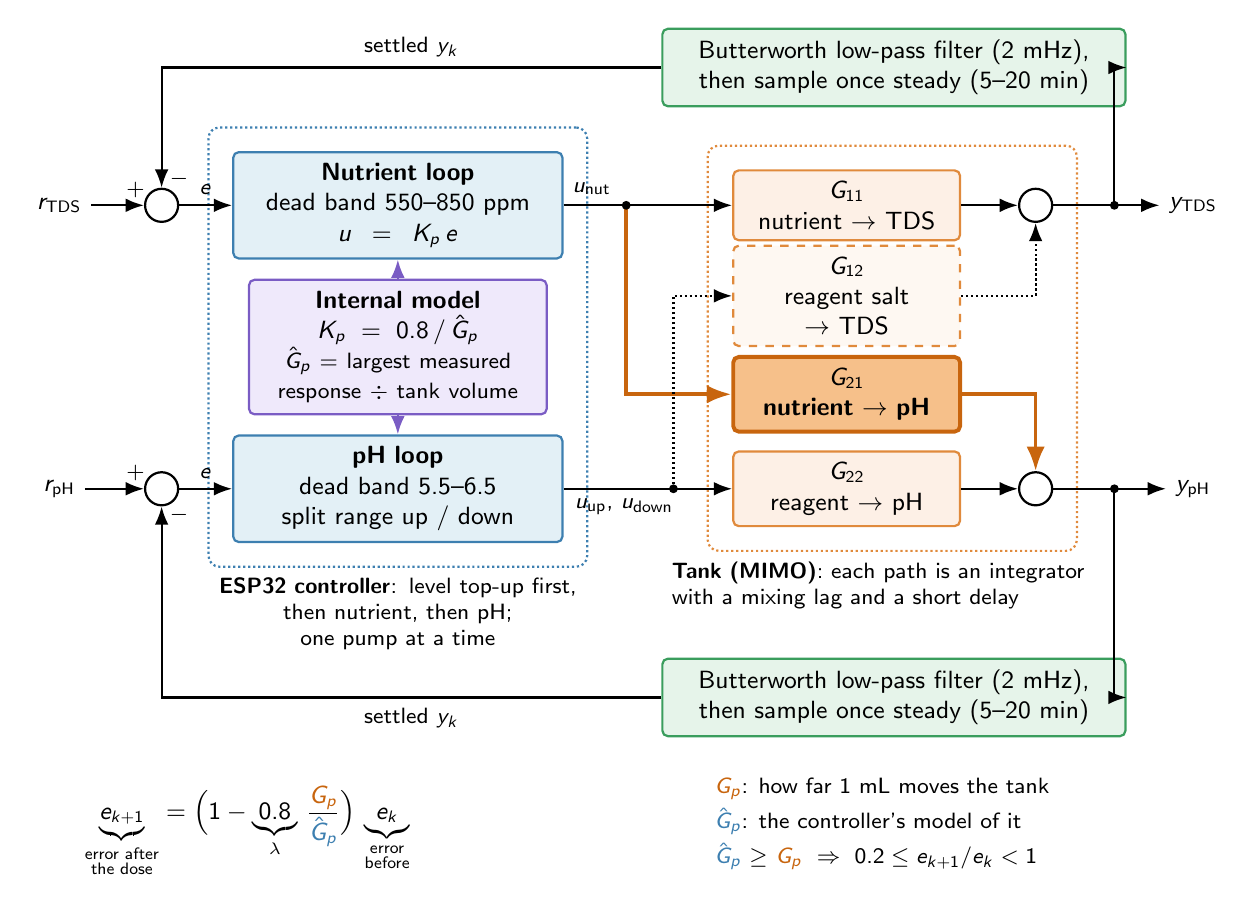
\begin{tikzpicture}[
    >=Latex, font=\small,
    box/.style={draw, rounded corners=2pt, thick, align=center, inner sep=4pt},
    ctrlbox/.style={box, fill=ctrl, draw=ctrledge, text width=3.9cm, minimum height=1.25cm},
    modelbox/.style={box, fill=model, draw=modeledge, text width=3.5cm},
    plantbox/.style={box, fill=plant, draw=plantedge, text width=2.6cm, minimum height=0.85cm},
    sensebox/.style={box, fill=sense, draw=senseedge, text width=5.6cm},
    sum/.style={draw, thick, circle, minimum size=0.42cm, inner sep=0pt},
    arr/.style={-{Latex}, thick},
    lbl/.style={font=\footnotesize},
  ]
  % ---------------- controller (ESP32) ----------------
  \node (rtds) at (0, 5.0) {$r_{\mathrm{TDS}}$};
  \node[sum] (s1) at (1.3, 5.0) {};
  \node[ctrlbox] (nut) at (4.3, 5.0) {\textbf{Nutrient loop}\\dead band 550--850 ppm\\$u = K_p\,e$};
  \node[modelbox] (mod) at (4.3, 3.2) {\textbf{Internal model}\\$K_p = 0.8\,/\,\hat G_p$\\\footnotesize $\hat G_p$ = largest measured\\response $\div$ tank volume};
  \node[ctrlbox] (ph) at (4.3, 1.4) {\textbf{pH loop}\\dead band 5.5--6.5\\split range up / down};
  \node (rph) at (0, 1.4) {$r_{\mathrm{pH}}$};
  \node[sum] (s2) at (1.3, 1.4) {};

  % ---------------- tank (MIMO) ----------------
  \node[plantbox] (g11) at (10.0, 5.0) {$G_{11}$\\nutrient $\to$ TDS};
  \node[plantbox, dashed, fill=plant!50] (g12) at (10.0, 3.85) {$G_{12}$\\reagent salt $\to$ TDS};
  \node[plantbox, fill=hot, draw=hotedge, line width=1.4pt] (g21) at (10.0, 2.6) {$G_{21}$\\\textbf{nutrient $\to$ pH}};
  \node[plantbox] (g22) at (10.0, 1.4) {$G_{22}$\\reagent $\to$ pH};
  \node[sum] (p1) at (12.4, 5.0) {};
  \node[sum] (p2) at (12.4, 1.4) {};
  \node (ytds) at (14.4, 5.0) {$y_{\mathrm{TDS}}$};
  \node (yph) at (14.4, 1.4) {$y_{\mathrm{pH}}$};
  \coordinate (b1) at (13.4, 5.0);
  \coordinate (b2) at (13.4, 1.4);

  % ---------------- measurement ----------------
  \node[sensebox] (f1) at (10.6, 6.75) {Butterworth low-pass filter (2 mHz),\\then sample once steady (5--20 min)};
  \node[sensebox] (f2) at (10.6, -1.25) {Butterworth low-pass filter (2 mHz),\\then sample once steady (5--20 min)};

  % ---------------- forward paths ----------------
  \draw[arr] (rtds) -- (s1);
  \draw[arr] (s1) -- node[above, lbl] {$e$} (nut);
  \draw[arr] (rph) -- (s2);
  \draw[arr] (s2) -- node[above, lbl] {$e$} (ph);
  \draw[arr, modeledge] (mod) -- (nut);
  \draw[arr, modeledge] (mod) -- (ph);
  % nutrient dose: to TDS, and (highlighted) to pH
  \coordinate (jn) at (7.2, 5.0);
  \draw[thick] (nut.east) -- node[above, lbl, pos=0.45] {$u_{\mathrm{nut}}$} (jn);
  \draw[arr] (jn) -- (g11);
  \draw[arr, hotedge, line width=1.3pt] (jn) |- (g21.west);
  \fill (jn) circle (1.6pt);
  % pH reagent: to pH, and (weak, dotted) its salt to TDS
  \coordinate (jp) at (7.8, 1.4);
  \draw[thick] (ph.east) -- node[below, lbl, pos=0.55] {$u_{\mathrm{up}},\,u_{\mathrm{down}}$} (jp);
  \draw[arr] (jp) -- (g22);
  \draw[arr, densely dotted] (jp) |- (g12.west);
  \fill (jp) circle (1.6pt);
  % summing into the outputs
  \draw[arr] (g11) -- (p1);
  \draw[arr, densely dotted] (g12.east) -| (p1.south);
  \draw[arr] (g22) -- (p2);
  \draw[arr, hotedge, line width=1.3pt] (g21.east) -| (p2.north);
  \draw[thick] (p1) -- (b1); \draw[arr] (b1) -- (ytds);
  \draw[thick] (p2) -- (b2); \draw[arr] (b2) -- (yph);
  \fill (b1) circle (1.6pt); \fill (b2) circle (1.6pt);

  % ---------------- feedback ----------------
  \draw[arr] (b1) |- (f1.east);
  \draw[arr] (f1.west) -| node[above, lbl, pos=0.25] {settled $y_k$} (s1.north);
  \draw[arr] (b2) |- (f2.east);
  \draw[arr] (f2.west) -| node[below, lbl, pos=0.25] {settled $y_k$} (s2.south);

  % ---------------- signs ----------------
  \node[lbl] at ([xshift=-0.33cm, yshift=0.2cm]s1) {$+$};
  \node[lbl] at ([xshift=0.22cm, yshift=0.33cm]s1) {$-$};
  \node[lbl] at ([xshift=-0.33cm, yshift=0.2cm]s2) {$+$};
  \node[lbl] at ([xshift=0.22cm, yshift=-0.33cm]s2) {$-$};

  % ---------------- grouping ----------------
  \begin{scope}[on background layer]
    \node[draw=ctrledge, densely dotted, thick, rounded corners, inner sep=0.3cm,
      fit=(nut)(mod)(ph), label={[lbl, align=center, text width=5.2cm]below:
      \textbf{ESP32 controller}: level top-up first,\\then nutrient, then pH; one pump at a time}] {};
    \node[draw=plantedge, densely dotted, thick, rounded corners, inner sep=0.3cm,
      fit=(g11)(g12)(g21)(g22)(p1)(p2), label={[lbl, align=left, text width=5.6cm]below:
      \textbf{Tank (MIMO)}: each path is an integrator\\with a mixing lag and a short delay}] {};
  \end{scope}

  % ---------------- why it cannot overshoot ----------------
  \node[anchor=north west, align=left] at (0.2, -2.25) {%
    $\displaystyle
    \underbrace{e_{k+1}}_{\substack{\text{error after}\\\text{the dose}}}
    = \Bigl(1 - \underbrace{0.8}_{\lambda}\,
      \frac{\color{gp}G_p}{\color{gphat}\hat G_p}\Bigr)\,
    \underbrace{e_k}_{\substack{\text{error}\\\text{before}}}$};
  \node[anchor=north west, align=left, lbl] at (8.2, -2.15) {%
    {\color{gp}$G_p$}: how far 1 mL moves the tank\\[2pt]
    {\color{gphat}$\hat G_p$}: the controller's model of it\\[2pt]
    {\color{gphat}$\hat G_p$} $\ge$ {\color{gp}$G_p$} $\;\Rightarrow\;$
    $0.2 \le e_{k+1}/e_k < 1$};
\end{tikzpicture}
\end{document}
